\chapter{Proof of Concept}
\label{ch:proof-of-concept}
Dit hoofdstuk bevat een vergelijkend experiment tussen twee open source serverless (FaaS) frameworks, namelijk Fission, dat werd aangegeven door Nubera en OpenFaaS. In dit onderdeel worden de twee frameworks opgezet op een Kubernetes cluster die bestaat uit één node. Beide frameworks worden opgezet op een MacBook Pro waarop Minikube draait. Minikube is een ''Out-of-the-box'' Kubernetes cluster die overal kan draaien. Er wordt gekozen om gebruik te maken van Minikube omdat op deze manier beide frameworks op identiek dezelfde hardware kunnen gedraaid worden. Daarnaast biedt Minikube dezelfde functionaliteiten als een volledige Kubernetes cluster die elders is opgezet. Dit hoofdstuk is opgedeeld in twee grote onderdelen waarbinnen telkens dezelfde secties met dezelfde stappen voor elk framework terug te vinden zijn. Daarnaast is er eveneens een sectie in dit hoofdstuk terug te vinden waarin de demofunctie, die serverless gedraaid zal worden op de frameworks, wordt voorgesteld. De demo bestaat uit het deployen van een Python functie die de functionaliteit van beide frameworks demonstreert en de executietijd van de functie meet. Later wordt er in dit onderzoek een vergelijking tussen Fission en OpenFaaS gemaakt waarbij onder meer gekeken zal worden naar het verschil in executietijd tussen de geschreven functie, de tijd die de volledige functie in beslag neemt (vanaf dat het HTTP request wordt verzonden), alsook de gebruiksvriendelijkheid. Deze Proof of Concept moet meer inzicht geven in beide frameworks en geeft een duidelijk beeld van wat deze precies inhouden. Merk op dat de opstelling van deze PoC enkel voor testing is en dus niet geschikt is voor productie. Indien dit in productie wordt overgenomen dan dienen er enkele additionele veiligheidsmaatregelen getroffen te worden maar daar wordt in dit onderzoek niet op verder gegaan.
\\\\
\section{Voorbereiding omgeving}
\label{sec:voorbereiding-omgeving}
\subsection{Onderliggende hardware}
Het experiment zal worden uitgevoerd op een MacBook Pro, model 2018 met volgende specificaties:
\begin{itemize}
    \item Processor: 2,2 GHz Intel Core i7
    \item Memory: 16 GB 2400 MHz DDR4
    \item Graphics: Radeon Pro 555X 4 GB en Intel UHD Graphics 630 1536 MB
    \item Opslag: 256 GB SSD
\end{itemize}

\subsection{Packet manager}
Om de opstelling van het experiment klaar te zetten is het zinvol gebruik te maken van Homebrew\footnote{https://brew.sh/}, dit is een packetmanager ontwikkeld voor macOS. Homebrew zorgt ervoor dat softwarepakketten kunnen worden gedownload uit bestaande repositories. In de verdere uitwerking van dit onderzoek wordt Homebrew eveneens gebruikt voor het installeren van software.\\\\
Homebrew kan worden geïnstalleerd door volgend commando in de Terminal uit te voeren: 
\begin{lstlisting}[language=bash]
$ /usr/bin/ruby -e "$(curl -fsSL 
https://raw.githubusercontent.com/Homebrew/install/master/install)"
\end{lstlisting}

\subsection{Softwarepakketten}
Alvorens de frameworks kunnen worden opgezet moeten er reeds enkele softwarepakketten aanwezig zijn. Enerzijds is Docker nodig als container engine, anderzijds Kubernetes als container platform. Daarnaast is er ook een hypervisor nodig die het draaien van een Minikube cluster mogelijk maakt. In dit onderzoek wordt gebruik gemaakt van VirtualBox als hypervisor, deze is open source en gratis. De softwarepakketten kunnen als volgt geïnstalleerd worden met Homebrew:        
\begin{lstlisting}[language=bash]
$ brew tap caskroom/cask
$ brew cask install virtualbox
$ brew cask install docker
$ brew cask install minikube
$ brew install kubernetes-cli
\end{lstlisting}

\section{Python demofunctie}
\label{sec:python-demofunctie}
Aan de hand van een zelfgeschreven Python functie zal de werking van beide frameworks worden gedemonstreerd. De demofunctie is eenvoudig en bestaat uit een print statement dat de gebruiker verwelkomt, vervolgens wordt er een loop uitgevoerd die ervoor zorgt dat de functie toch even loopt en uiteindelijk wordt deze uitvoeringstijd weggeschreven naar een Google Spreadsheet bestand. De Python functie maakt gebruik van de Google API voor het wegschrijven naar het spreadsheet bestand. De functie wordt verpakt in een Docker image zodat deze naadloos kan worden gedeployed op beide frameworks. De Docker image met de functie is gepubliceerd op de Docker Hub repository van Lennert Mertens (private repository). Om gebruik te kunnen maken van Google spreadsheets moet er een Google project worden aangemaakt via de Google API, deze stappen staan verder beschreven. Er wordt gekozen voor dit soort functie zodat er later in dit onderzoek een besluit kan worden gevormd over welk framework de snelste executie van functies biedt. Het ultieme doel is dat de data in het Google bestand kan worden geanalyseerd en vergeleken. Elke demo start met een leeg werkblad zodat de resultaten die werden weggeschreven toepasbaar zijn op het specifieke framework dat werd getest.

\subsection{Google API}
De Python functie schrijft de executietijd van de functies weg naar een bestand op Google spreadsheets. Om gebruik te maken van een spreadsheet bestand moet eerst de API worden geconfigureerd, daarnaast moeten ook de credentials op de demo machine worden geconfigureerd. Het Goolge project wordt opgezet zodat de functie data kan wegschrijven naar de spreadsheet, in sectie \ref{sec:google-api} is een gedetailleerd stappenplan terug te vinden voor het instellen van de Google API in combinatie met Google spreadsheets. Om gebruik te maken van Google API features moeten oauth2client, gspread en google-api-python-client geïnstalleerd worden. De drie packages die nodig zijn voor de uitvoer van de functie worden gebundeld in een tekstbestand ''requirements.txt'', dit bestand kan vervolgens door ''pip'' worden gebruikt voor de installatie van de softwarepakketten, het bestand is terug te vinden in bijlage \ref{sec:requirements.txt}.

\newpage
\subsection{Code demofunctie}
\label{sec:demofunctie}
\begin{lstlisting}[language=python]
import time
import gspread
from oauth2client.service_account import ServiceAccountCredentials

# Function to get the first empty row in Gooogle Spreadsheet
def next_available_row(worksheet):
      str_list = filter(None, worksheet.col_values(1)) 
      return str(len(str_list)+1)

# Initialize variables for Google API
scope = ['https://spreadsheets.google.com/feeds',
         'https://www.googleapis.com/auth/drive']
credentials = ServiceAccountCredentials
              .from_json_keyfile_name('credentials.json', scope)
client = gspread.authorize(credentials)
worksheet = client.open("executietijd-openfaas").sheet1
next_row = next_available_row(worksheet)

# Start timer 
start = time.time()

# Print message visible by users
print("Hello everyone, this is a serverless demo function!")

# Start loop function to measure execution time
a = range(1000000)
b = []
for i in a:
     b.append(i*2)

# Stop timer
end = time.time()

# Calculate the execution time of the function in seconds
execution_time= end - start

# Write the execution time to Google spreadsheet
worksheet.update_acell("A{}".format(next_row), execution_time)
\end{lstlisting}

\newpage
\section{OpenFaaS}
Het eerste framework dat wordt uitgetest is OpenFaaS. Het experiment wordt opgezet op een MacBook Pro die voldoet aan voorgaande specificaties en beschikt over de benodigde softwarepakketten zoals eerder ook beschreven werd. De stappen die doorlopen worden in het opzetten en uitvoeren van het experiment, zijn steeds duidelijk gedocumenteerd en staan chronologisch gerangschikt. De installatieprocedure is eenvoudig te volgen en is reproduceerbaar aan de hand van de gedocumenteerde stappen en bijhorende scripts.

\subsection{Configuratie Minikube}
\label{sec:configuratie-minikube}
Vooraleer OpenFaaS geïnstalleerd kan worden, wordt er een lokale Kubernetes cluster die bestaat uit één node opgezet met Minikube. Een Minikube cluster biedt dezelfde functionaliteiten als een productieomgeving waarop een Kubernetes cluster is geïnstalleerd. Er wordt gebruik gemaakt van Kubernetes als container orchestrator. Een orchestrator is een tool die instaat voor het management van containers en microservice applicaties. Kubernetes zorgt ervoor dat applicaties schaalbaar kunnen worden opgezet, staat in voor het volledige beheer van de containers en voorziet ''High-availability''.
\\
In sectie \ref{sec:voorbereiding-omgeving} werden de benodigde softwarepakketten reeds geïnstalleerd. Indien alle stappen succesvol werden doorlopen dan kan de Minikube cluster probleemloos als volgt worden gestart. Na de installatie wordt eerst ook de status van de cluster nagegaan. De Minikube cluster wordt opgezet met aangepaste specificaties, zijnde: CPUs=4, Memory=8192MB, Disk=20000MB.

\begin{lstlisting}[language=bash]
$ minikube start --cpus 4 --memory 8192
$ minikube status
\end{lstlisting}

De uitvoer van het tweede commando geeft een overzicht dat er als volgt zou moeten uitzien, het IP adres wijkt mogelijks af van hetgene in de output. Wanneer de output overeenkomt met deze dan is Minikube succesvol geïnstalleerd.
\begin{lstlisting}[language=bash]
host: Running
kubelet: Running
apiserver: Running
kubectl: Correctly Configured: pointing to \ 
minikube-vm at 192.168.99.107
\end{lstlisting}

\subsection{Installatie OpenFaaS}
Indien de installatie van Minikube uit voorgaande sectie succesvol is, dan kan OpenFaaS worden geïnstalleerd. De installatie van OpenFaaS bestaat uit enkele stappen die werden omgevormd tot een shell script. Het is mogelijk dit script vanuit de Terminal uit te voeren, vervolgens start de installatie van OpenFaaS. De volledige installatie van het framework is geautomatiseerd en reproduceerbaar. Het script is terug te vinden als bijlage \ref{sec:installatie-openfaas} onder de naam Installatiescript OpenFaaS. De installatie is gebaseerd op een blogpost van \textcite{Ellis2017}, de founder van OpenFaaS. In de documentatie van OpenFaaS\footnote{https://docs.openfaas.com/} wordt eveneens naar deze blogpost gerefereerd als installatiehandleiding. Na de  uitvoering van het script is OpenFaaS geïnstalleerd bovenop de Minikube cluster. Na de installatie worden enkele artefacten geproduceerd die communicatie met het framework mogelijk maken.
\\
\begin{itemize}
    \item OpenFaaS UI standaard poort: 31112
    \item OpenFaaS UI URL: http://MINIKUBE-IP:31112/ui/
\end{itemize}
 
\subsection{Gebruik OpenFaaS}
\subsubsection{User Interface}
Na de installatie is het mogelijk naar de OpenFaaS UI te surfen, \\bijvoorbeeld: http://192.168.99.107:31112. 
De eerste keer dient er aangemeld te worden met gebruiker ''admin'' (Deze gebruiker wordt aangemaakt in het installatiescript) en het wachtwoord dat in de Terminal werd weergegeven door het installatiescript. Na het aanmelden is de interface zoals in figuur \ref{fig:openfaas-ui} te zien. De UI ziet er vrij sober uit na installatie, er is eveneens een mogelijkheid om een nieuwe functie te deployen via de ''Deploy New Function'' knop. Wanneer gebruikers kiezen een nieuwe functie te deployen dan kunnen ze enerzijds kiezen voor een community functie, dit zijn reeds bestaande functies die op het OpenFaaS framework kunnen gedraaid worden. Anderzijds kunnen gebruikers ook manueel zelfgeschreven functies deployen aan de hand van deze interface. In dit onderzoek worden functies gedeployed via de command line met het faas-cli commando. Deployments van functies via de command line biedt een betere reproduceerbaarheid en is vaak sneller en makkelijker te reproduceren. Er wordt ook bewust gekozen voor de command line tools omdat niet alle serverless frameworks over een UI beschikken. De interface is een leuke feature en is makkelijk in gebruik voor mensen die aan de slag willen met serverless, deze wordt eveneens standaard meegeïnstalleerd met OpenFaaS.
\begin{figure}
    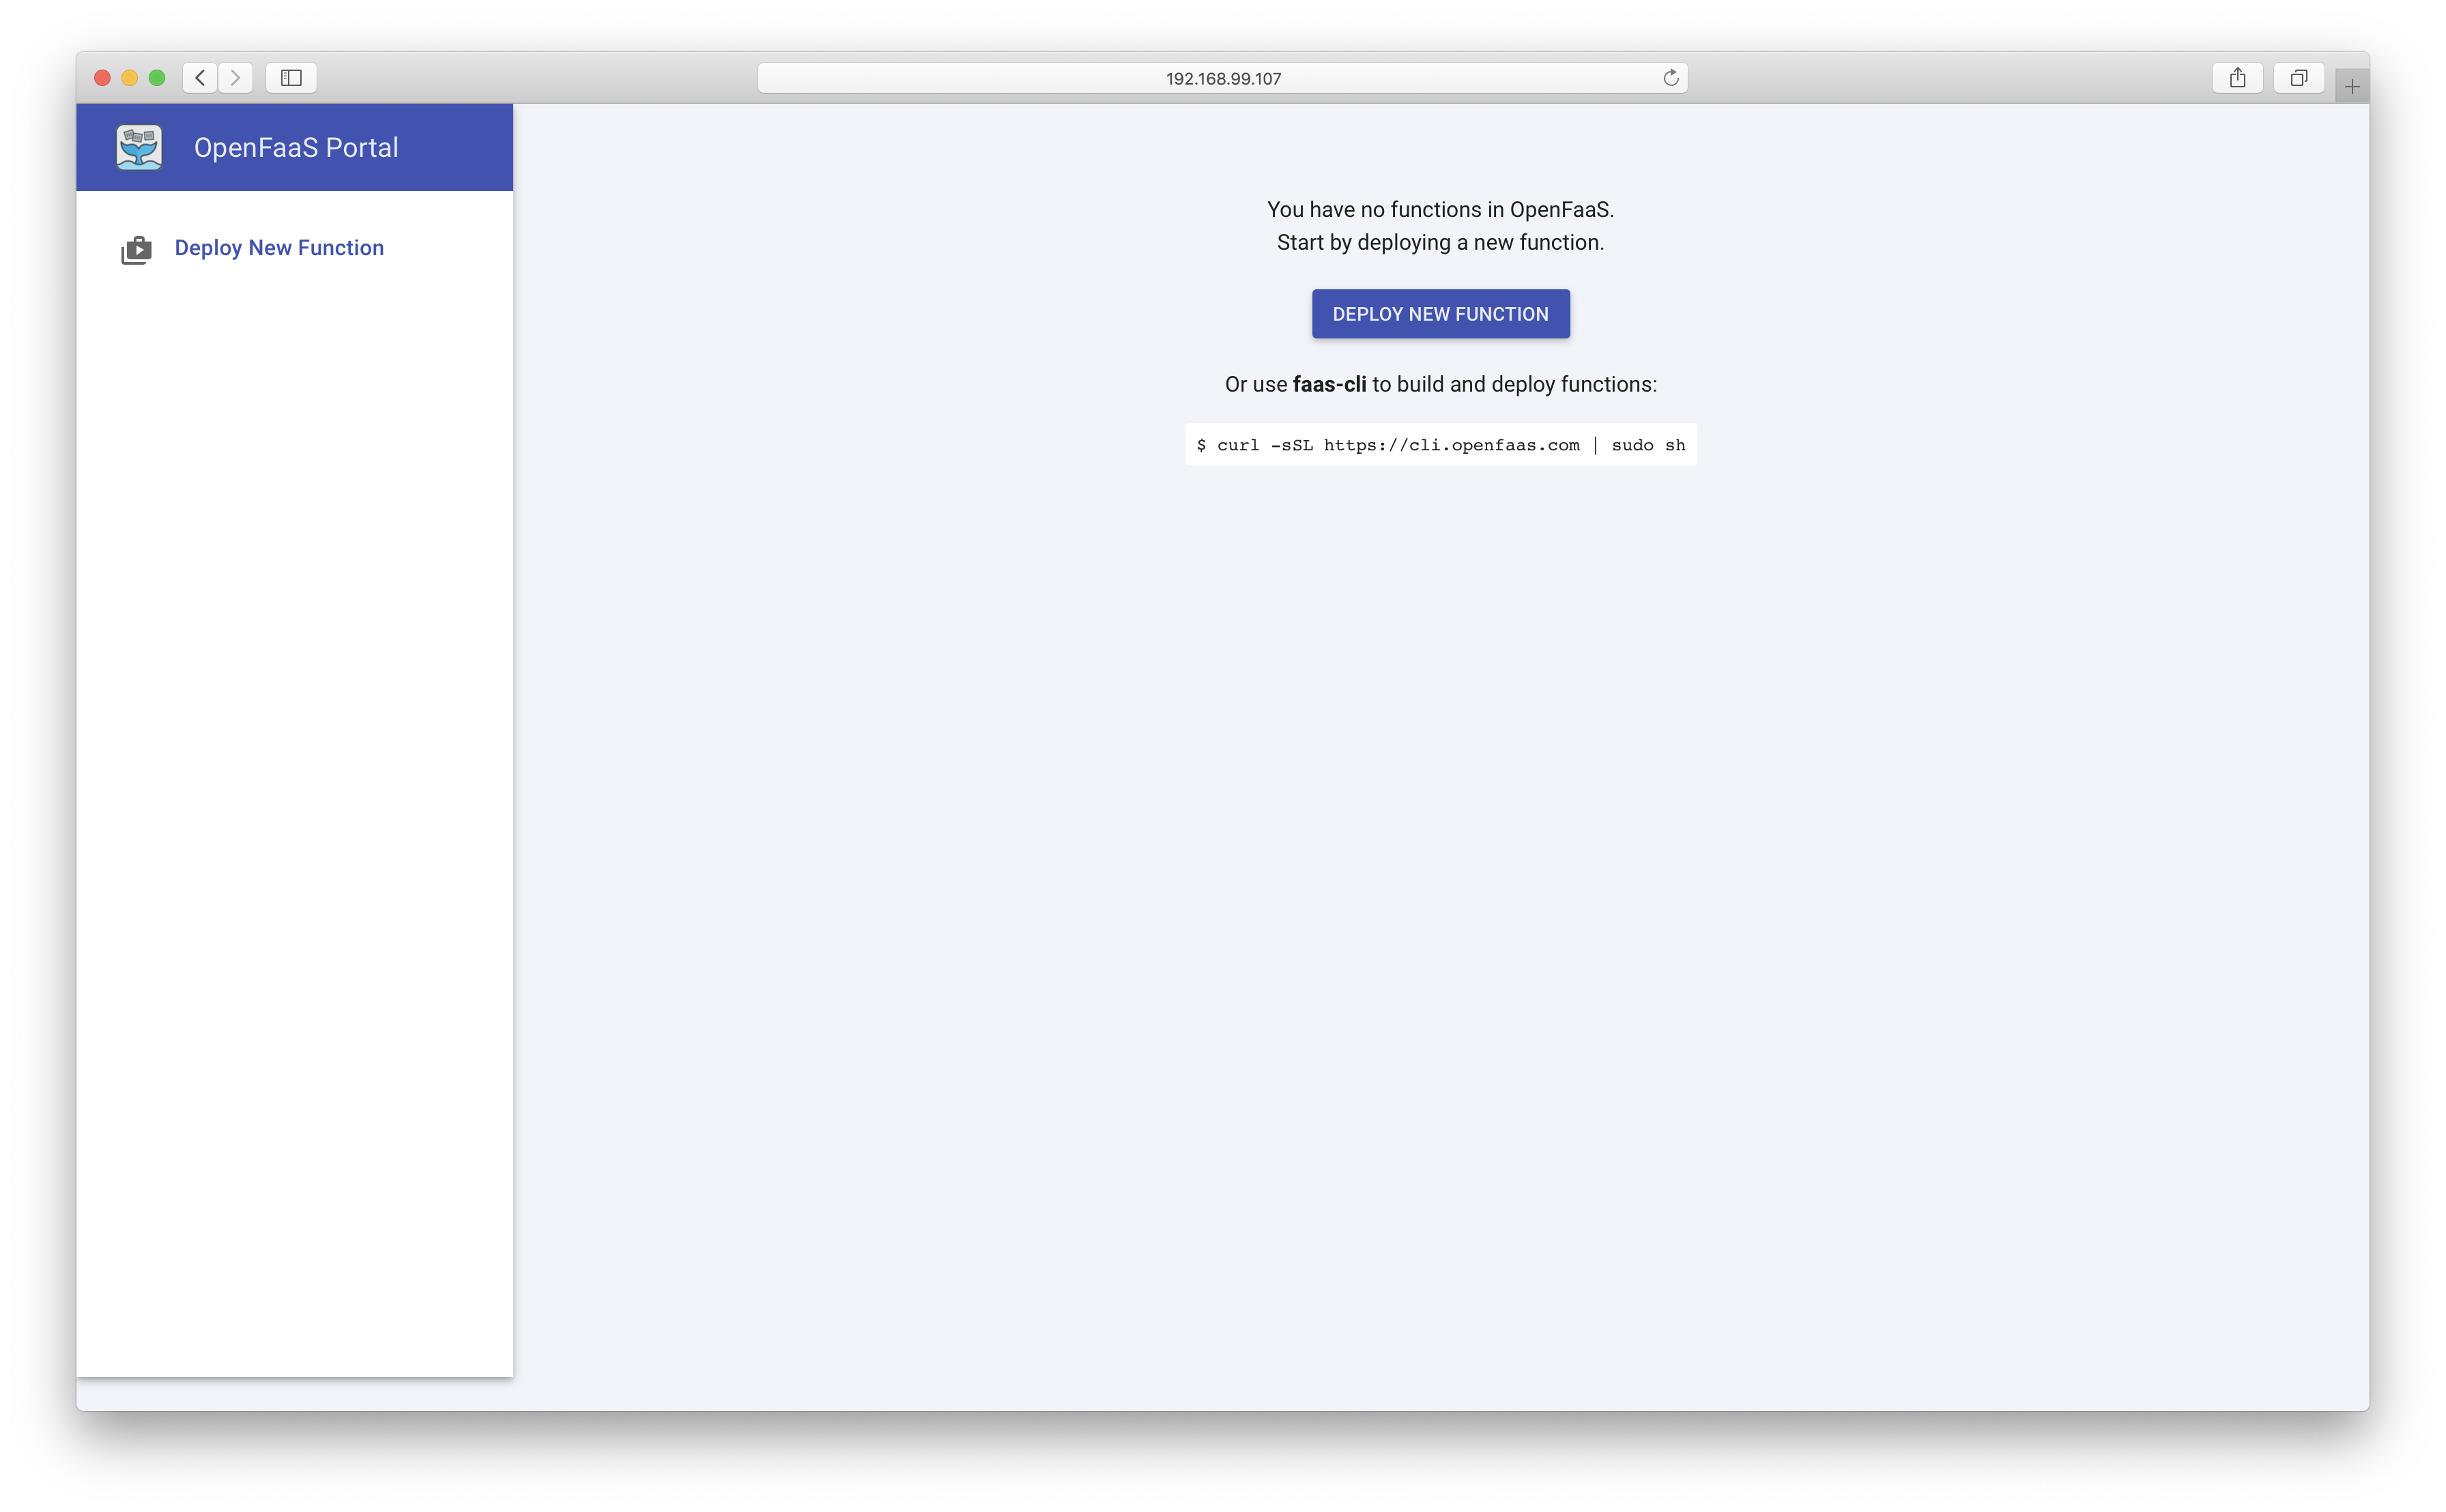
\includegraphics[width=1\textwidth]{img/openfaas-ui.png}
    \caption{OpenFaaS User Interface}
    \label{fig:openfaas-ui}  
\end{figure}

\subsubsection{Command line tools}
Faas-cli is de command line tool die beheer van OpenFaaS voorziet aan de hand van de console. Vooraleer van start te kunnen gaan moet de gebruiker inloggen via de Terminal door volgend commando in te voeren. Het paswoord werd tijdens de installatie in de Terminal weggeschreven, net zoals het IP adres waarop OpenFaaS draait. Daarnaast beschikt de shell ook over environment parameters met het wachtwoord en de URL voor OpenFaaS.
\begin{lstlisting}[language=bash]
$ faas-cli login -g http://$OPENFAAS_URL -u admin -p $PASSWORD
\end{lstlisting}
De command line tools voorzien meer functionaliteiten dan de UI. Het is mogelijk om functies te deployen via de CLI, de omgeving te beheren, confidentiële sleutels en wachtwoorden te beheren etc.

\subsubsection{Prometheus monitoring}
OpenFaaS voorziet monitoring aan de hand van Prometheus, via een Grafana dashboard kunnen verschillende metrics van functies worden bekeken. De configuratie van het dashboard werd reeds voorzien in installatiescript \ref{sec:installatie-openfaas}. Na de configuratie van Prometheus en Grafana kan het dashboard worden geraadpleegd via de GRAFANA\_URL, bijvoorbeeld http://192.168.99.107:32548/dashboard/db/openfaas. In figuur \ref{fig:grafana-dashboard} is het Grafana dashboard zichtbaar dat wordt weergegeven bij het openen van de link. Alvorens dit scherm kan geraadpleegd worden dient de gebruiker in te loggen met de default gebruiker ''admin'' met wachtwoord ''admin''. Grafana is standaard beschikbaar in het installatiepakket van OpenFaaS en dient enkel geactiveerd te worden.
\begin{figure}
    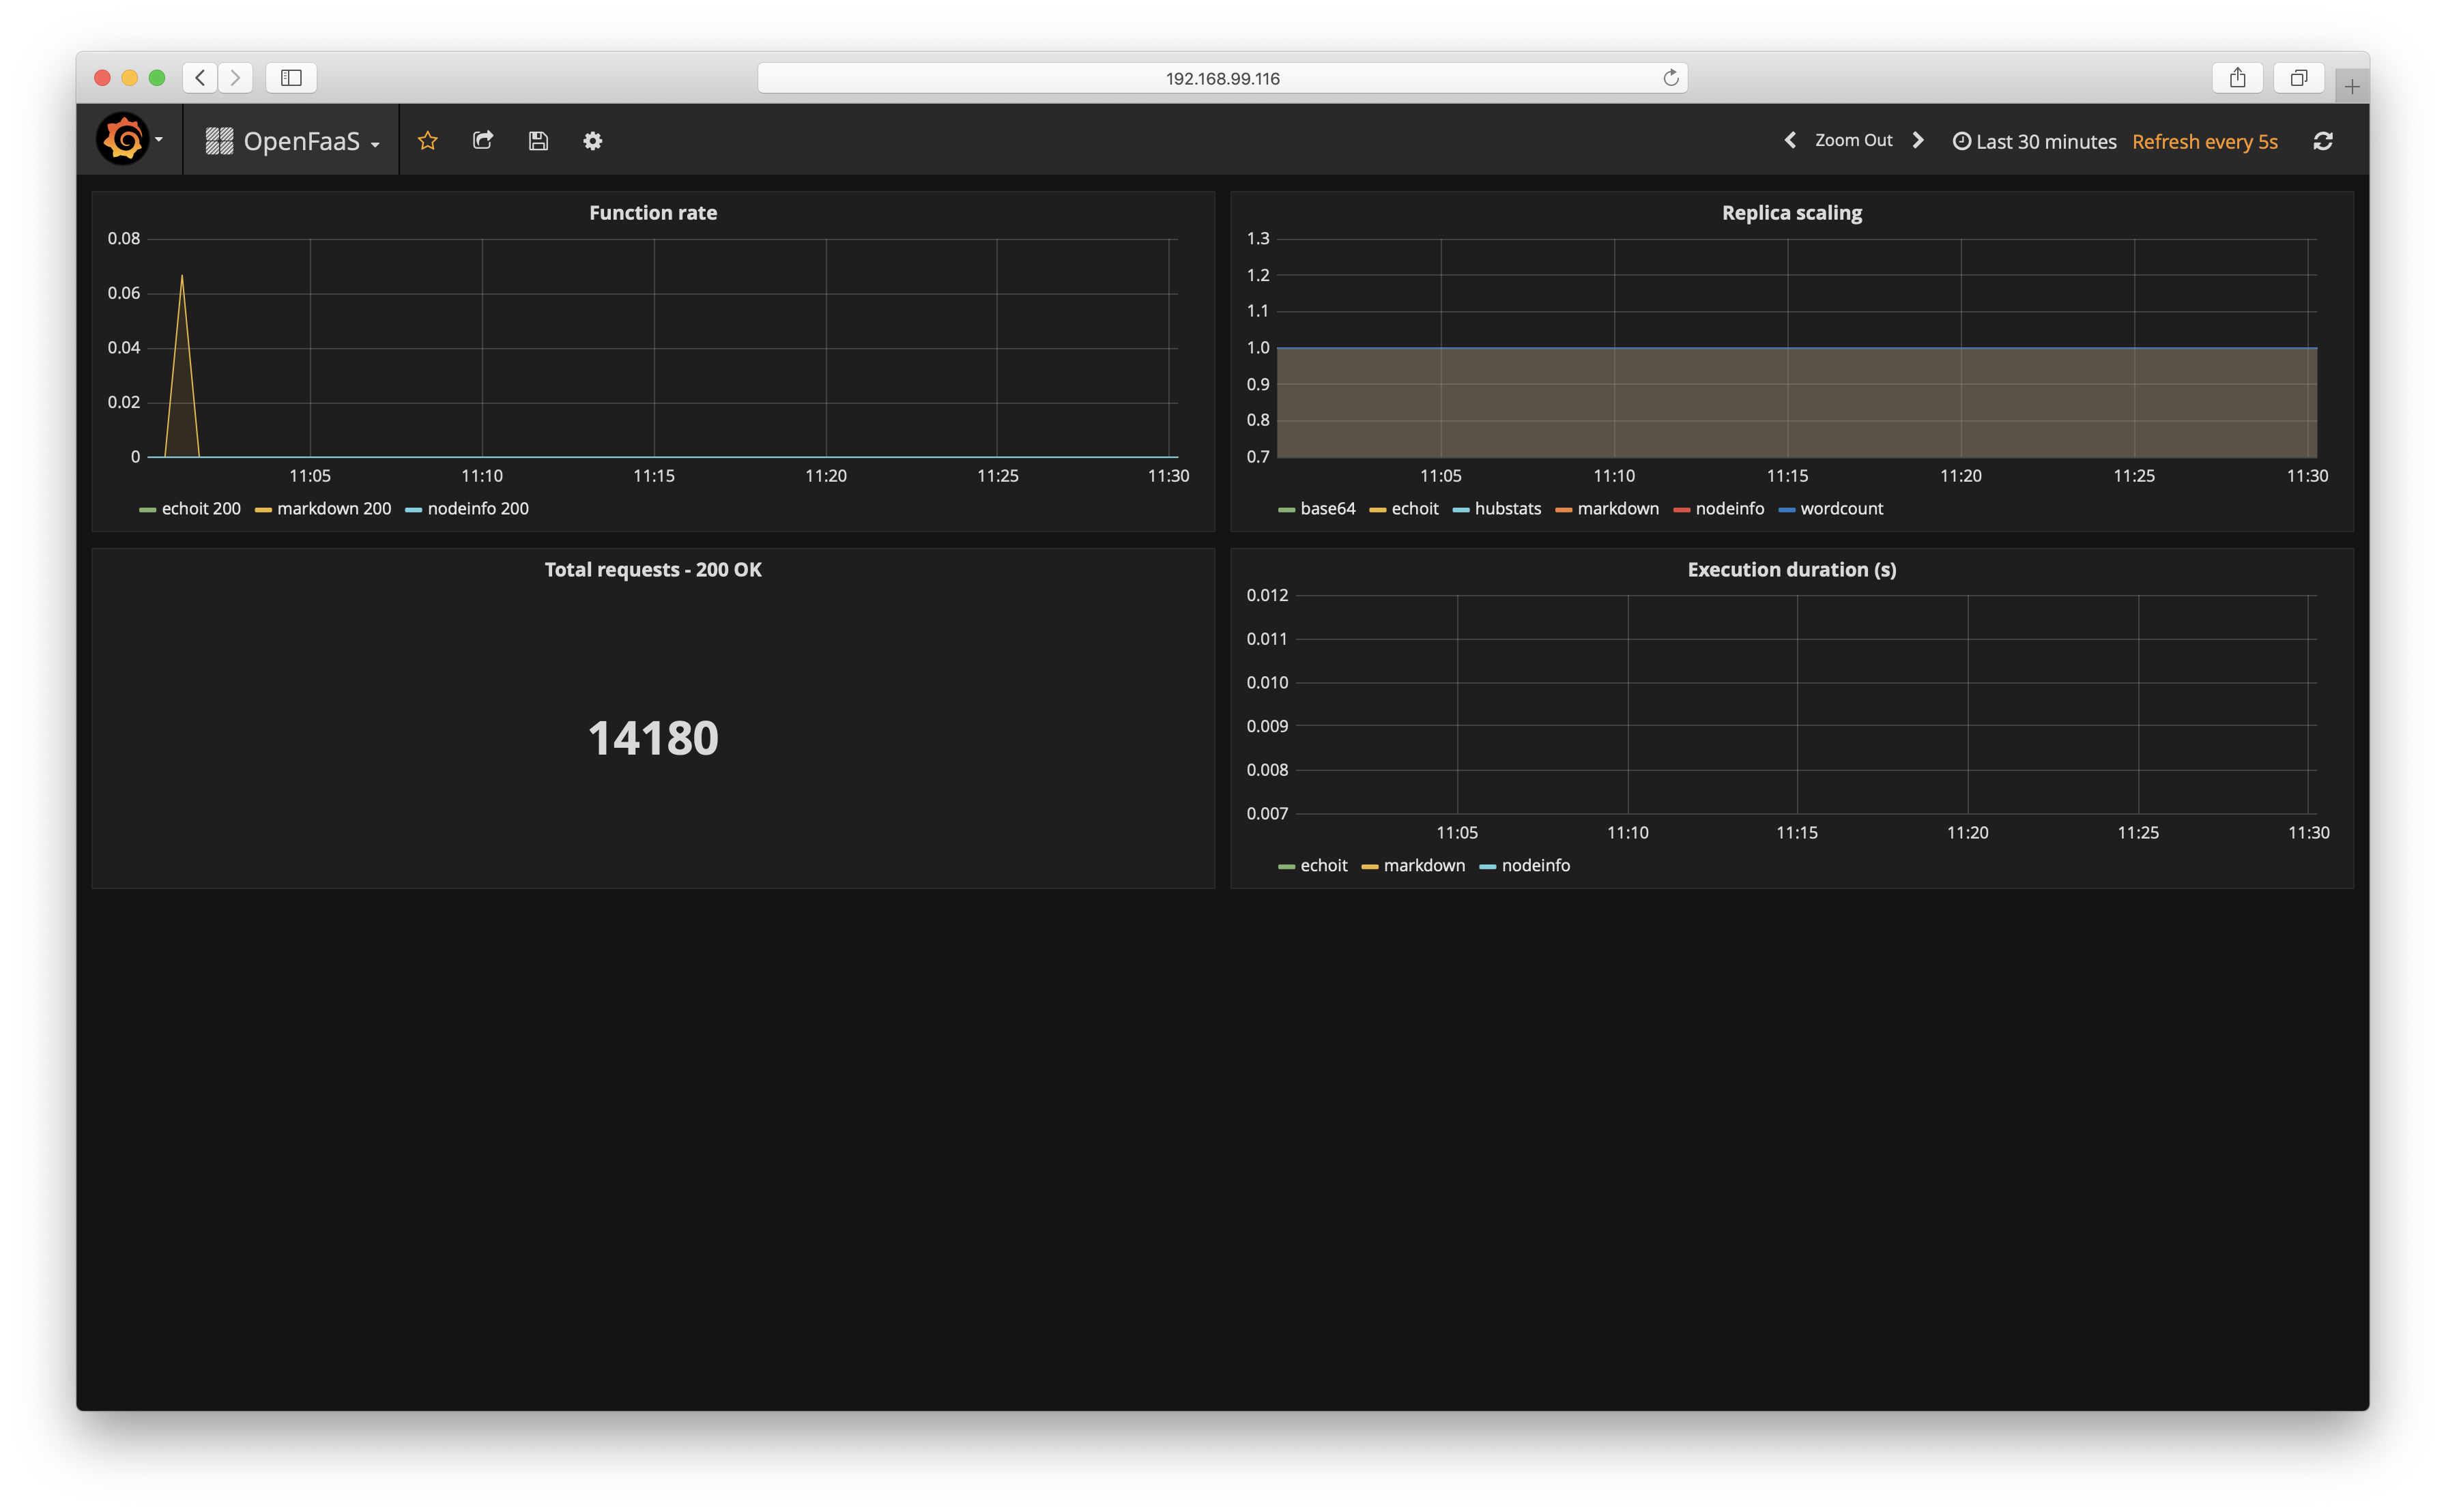
\includegraphics[width=1\textwidth]{img/grafana-dashboard.png}
    \caption{Grafana dashboard}
    \label{fig:grafana-dashboard}  
\end{figure}

\subsection{Deployment nieuwe demofunctie}
Het OpenFaaS framework wordt getest aan de hand van de zelfgeschreven functie die reeds beschreven is in sectie \ref{sec:python-demofunctie}. De functie wordt gedeployed aan de hand van de faas-cli tool. De code die werd geschreven wordt eveneens aangepast zodanig dat er gebruik kan worden gemaakt van Kubernetes secrets\footnote{https://docs.openfaas.com/reference/secrets/} voor het beheer van credentials die nodig zijn voor de Google API. Het deployen van een functie is slechts mogelijk indien alle voorgaande stappen succesvol werden uitgevoerd. Het deployen van de functie is onderverdeeld in verschillende stappen die hieronder uitgebreid worden beschreven.

\subsubsection{1. Aanmelden via faas-cli}
Indien er eerder nog niet werd ingelogd via de faas-cli dan moet dit gebeuren alvorens verder te gaan. Met behulp van volgend commando kan worden ingelogd, indien dit vanuit dezelfde shell als diegene waarin het installatiescript werd uitgevoerd gebeurt. Als de omgevingsvariabelen niet ingesteld zijn dan kunnen deze worden aangepast naar het IP adres en wachtwoord van het Tiller service account.
\begin{lstlisting}[language=bash]
$ faas-cli login -g http://$OPENFAAS_URL -u admin -p $PASSWORD
\end{lstlisting}

\subsubsection{2. Aanmaken Kubernetes secret}
Eerder werd er een credential account aangemaakt via Google Cloud API. De credentials die bij het aangemaakte account horen werden opgeslagen op een lokale locatie, deze credentials worden nu in een Kubernetes secret gestopt. OpenFaaS kan secrets uitlezen en deze gebruiken in functies, dit zorgt voor extra security, zo hoeven de credentials niet aanwezig te zijn in de Docker image van de functie.

\begin{lstlisting}[language=bash]
$ kubectl create secret generic secret-api-credentials \
 --from-file=secret-api-credentials=credentials-serverless.json \
 --namespace openfaas-fn
\end{lstlisting}

\subsubsection{3. Deploy functie}
De eerste keer dat de gebruiker een functie wilt deployen moeten er enkele stappen worden genomen, de functie moet worden geschreven, een YAML bestand met parameters specifiek voor deployment moet worden gemaakt en de gebruiker moet inloggen op Docker Hub voor het publiceren van Docker images. Wanneer een gebruiker een functie maakt, dan wordt deze op Docker Hub geplaats, vandaar het belang dat de gebruiker inlogt. Standaard zal een functie die wordt gedeployed een container opzetten die continue draait (standaard instelling), hierdoor kan er steeds snel op een request worden gereageerd en worden cold-start vermeden. Volgende stappen worden ondernomen wanneer de demofunctie voor het eerst wordt gedeployed.

\begin{lstlisting}[language=bash]
# 1. Login op Docker Hub.
$ docker login

# 2. Maak een nieuwe functie.
$ mkdir demo-functie; cd demo-functie

# serverless-demo is de naam die de functie zal krijgen,
# prefix is de gebruikersnaam op Docker Hub.

$ faas-cli new --lang python serverless-demo --prefix="lennertmertens"

# De inhoud van de map ziet eruit als volgt na uitvoer 
# van vorig commando.
$ ls
serverless-demo     serverless-demo.yml    template

# Vul de template bestanden aan naar eigen wensen en schrijf de functie
# De inhoud van de bestanden wordt hieronder weergegeven.

# 3. Build de functie die werd geschreven.
$ faas-cli build -f serverless-demo.yml

# 4. Push de Docker image van de functie naar Docker Hub.
$ faas-cli push -f serverless-demo.yml

# 5. Deploy de functie op het OpenFaaS framework.
$ faas-cli deploy -f serverless-demo.yml
\end{lstlisting}

De bestanden voor het maken en deployen van de functie zien er als volgt uit.

\subsubsection{serverless-demo.yml}
Aan de hand van dit bestand wordt de functie gedeployed. Dit bestand is een template waaraan enkele zaken zijn toegevoegd die specifiek zijn voor de demo-omgeving die werd opgezet. In bijlage \ref{sec:serverless-demo.yml} is de inhoud van dit bestand terug te vinden. De gateway is de URL van de OpenFaaS omgeving. De image is de Docker image dat wordt gebruikt voor het deployen van de functie op het framework. De ''secrets'' optie moet eveneens worden toegevoegd indien er gebruik wordt gemaakt van een Kubernetes secret, op die manier kan de functie de inhoud ervan opvragen.

\subsubsection{severless-demo/handler.py}
Onder de map serverless-demo is het handler.py bestand terug te vinden, dit is een Python script dat de functionaliteit bevat. Het Python bestand is de code die de functie vormt. In bijlage \ref{sec:demofunctie-openfaas} is de code te zien die specifiek voor deze opstelling wordt gebruikt

\subsubsection{serverless-demo/requirements.txt}
Onder de serverless-demo map is eveneens een requirements.txt bestand terug te vinden. Het bestand bevat de dependencies waar het Python script afhankelijk van is, dit zijn packages nodig om de functie uit te voeren. De packages staan opgelijst in bijlage \ref{sec:requirements.txt}.

\subsection{Deployment bestaande functie}
Wanneer de functie werd gebuild en in een repository op Docker Hub werd geplaatst dan volstaat het om enkel een template file te hebben zoals \ref{sec:serverless-demo.yml}. De functie wordt vanaf een bestaande image gedeployed dus het is niet meer nodig deze image opnieuw te builden. Images in Docker registries bieden de mogelijkheden dat ze eender waar kunnen worden gebruikt door iedereen of door een afgeschermde groep mensen. Het voordeel van serverless functies is dat er per functie een container wordt gebuild die alle dependencies en runtime voor een specifiek stuk code bevat.

\begin{lstlisting}[language=bash]
# Deploy bestaande functie op het OpenFaaS framework
$ faas-cli template pull
$ faas-cli deploy -f serverless-demo.yml
\end{lstlisting}

\subsection{Uitvoeren demofunctie}
\label{sec:openfaas-uitvoeren-functie}
De demofunctie reageert wanneer het een HTTP GET request ontvangt, deze actie kan worden getriggered op verschillende manieren. Via de UI is het mogelijk de functie aan te roepen door deze te selecteren en dan op de knop ''invoke'' te klikken, wanneer deze actie wordt uitgevoerd, wordt er een boodschap teruggegeven en eveneens werd de uitvoeringstijd van de functie weggeschreven naar het Google spreadsheet bestand. In figuur \ref{fig:openfaas-functie-ui} is de response van de functie zichtbaar, de overeenkomstige uitvoeringstijd van de functie (de tijd dat de code uitvoert en niet de tijd dat het duurt vanaf de request tot de response) werd weggeschreven naar het Google spreadsheet bestand.
De functie kan eveneens worden aangeroepen via het ''curl'' commando in de terminal.

\begin{lstlisting}[language=bash]
# Aanroep functie met curl.
 $ curl http://$OPENFAAS_URL/function/serverless-demo
\end{lstlisting}

\begin{figure}
    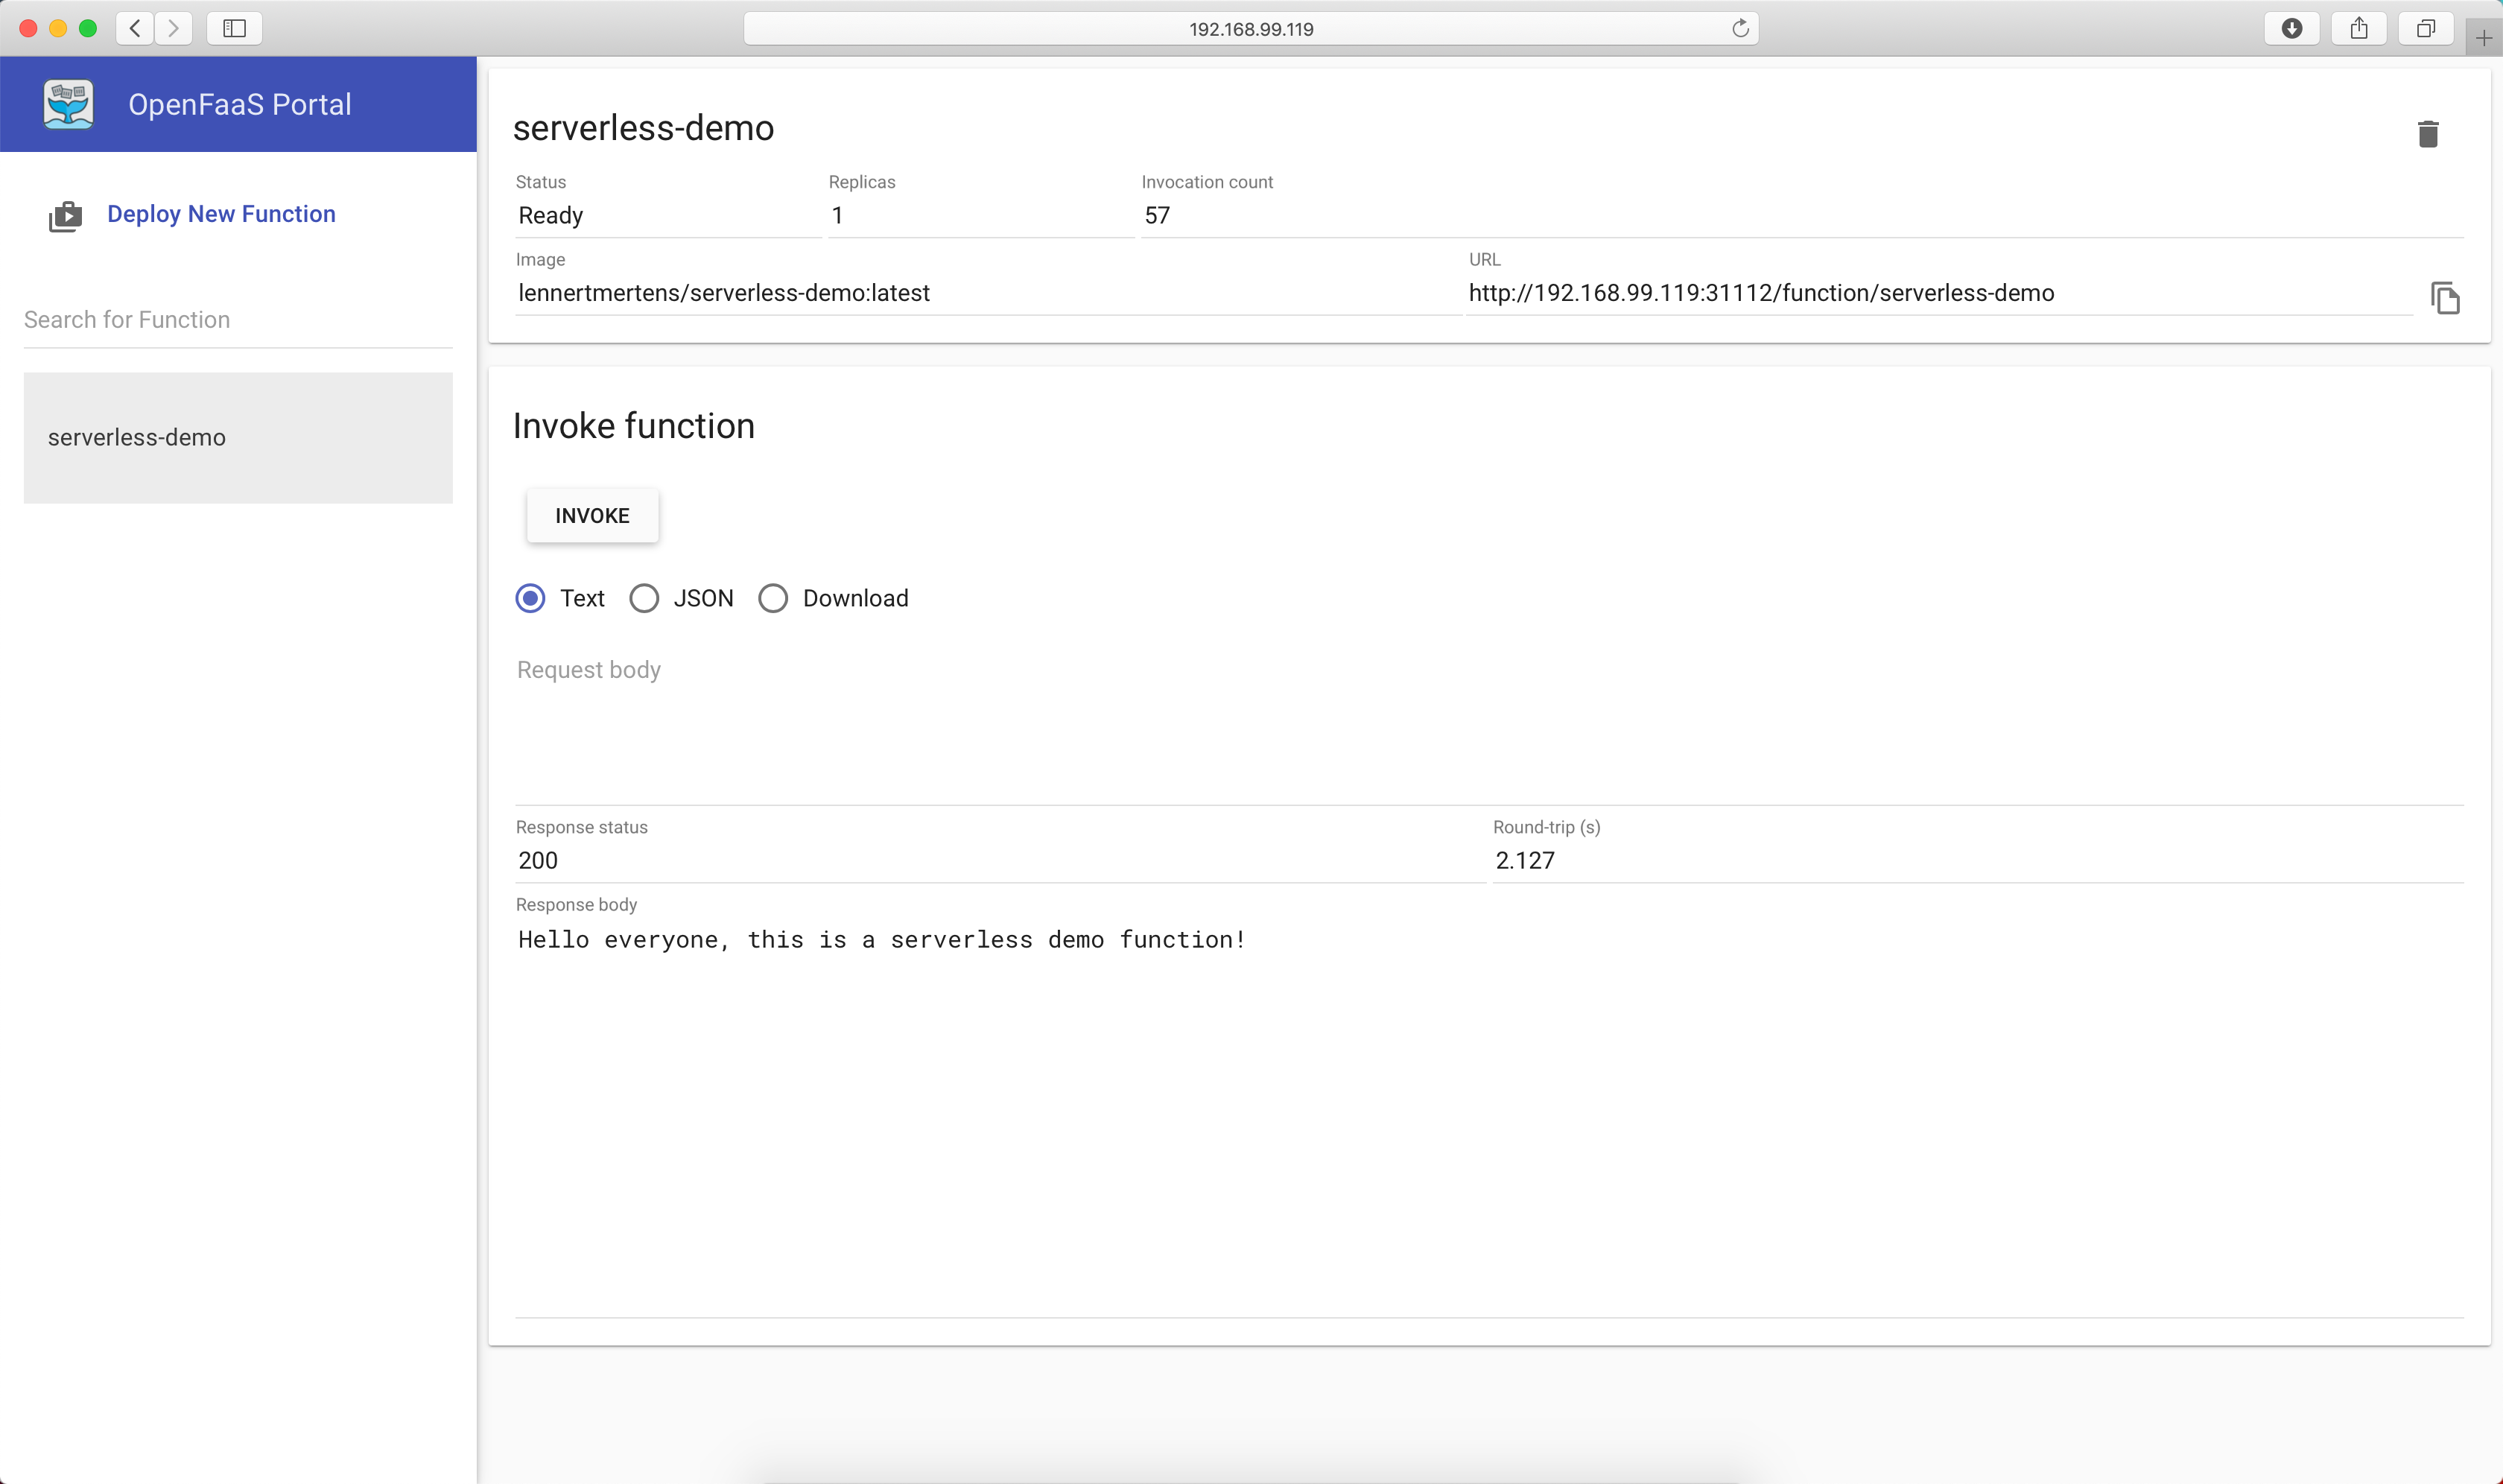
\includegraphics[width=1\textwidth]{img/openfaas-demo-ui.png}
    \caption{Aanroep OpenFaaS functie via UI.}
    \label{fig:openfaas-functie-ui}  
\end{figure}

\subsection{Schaalbaarheid OpenFaaS}
Een van de requirements waaraan het framework moet voldoen is automatische schaalbaarheid. Wanneer het aantal pods (dit is te vergelijken met één container in Kubernetes) van de functie wordt opgevraagd dan is er te zien dat er initieel maar één draait, zie figuur \ref{fig:openfaas-scalability-1}.
\begin{figure}
    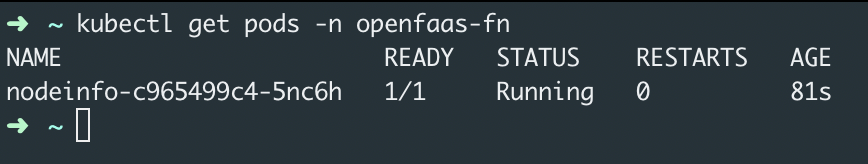
\includegraphics[width=1\textwidth]{img/openfaas-scalability-1.png}
    \caption{OpenFaaS standaard pods}
    \label{fig:openfaas-scalability-1}  
\end{figure}

Wanneer de functie zeer veel wordt aangeroepen aan de hand van bijvoorbeeld loop statements, dan zullen we zien dat wanneer we de pods opnieuw opvragen deze opschalen zonder dat hier iets moet voor worden gedaan. In figuur \ref{fig:openfaas-scalability-2} is te zien hoe de functie wordt aangeroepen en hoe de pods automatisch schalen. De functie die dit demonstreert is een eenvoudige functie\footnote{https://github.com/openfaas/faas/tree/master/sample-functions/NodeInfo} die informatie over de node ophaalt en deze teruggeeft aan de gebruiker, dit is een community functie die beschikbaar is in de OpenFaaS store en via de UI kan worden gedeployed. Hoe meer requests de functie moet verwerken, hoe meer pods er worden opgebracht. Als de requests worden gestopt dan schaalt OpenFaaS weer down zoals in figuur \ref{fig:openfaas-scalability-3} te zien is. Standaard zal er steeds een container blijven draaien, dit zorgt ervoor dat cold-starts worden vermeden. Er worden dus steeds een klein aantal resources verbruikt maar dit is een bewuste keuze omdat de container ervoor zorgt dat hoge latency wordt vermeden. In OpenFaaS kan de gebruiker zelf bepalen wanneer en hoe de functie moet geschaald worden, zo kan er ook gekozen worden om een container volledig af te zetten wanneer deze voor een bepaalde tijd geen requests ontvangt.

\begin{figure}
    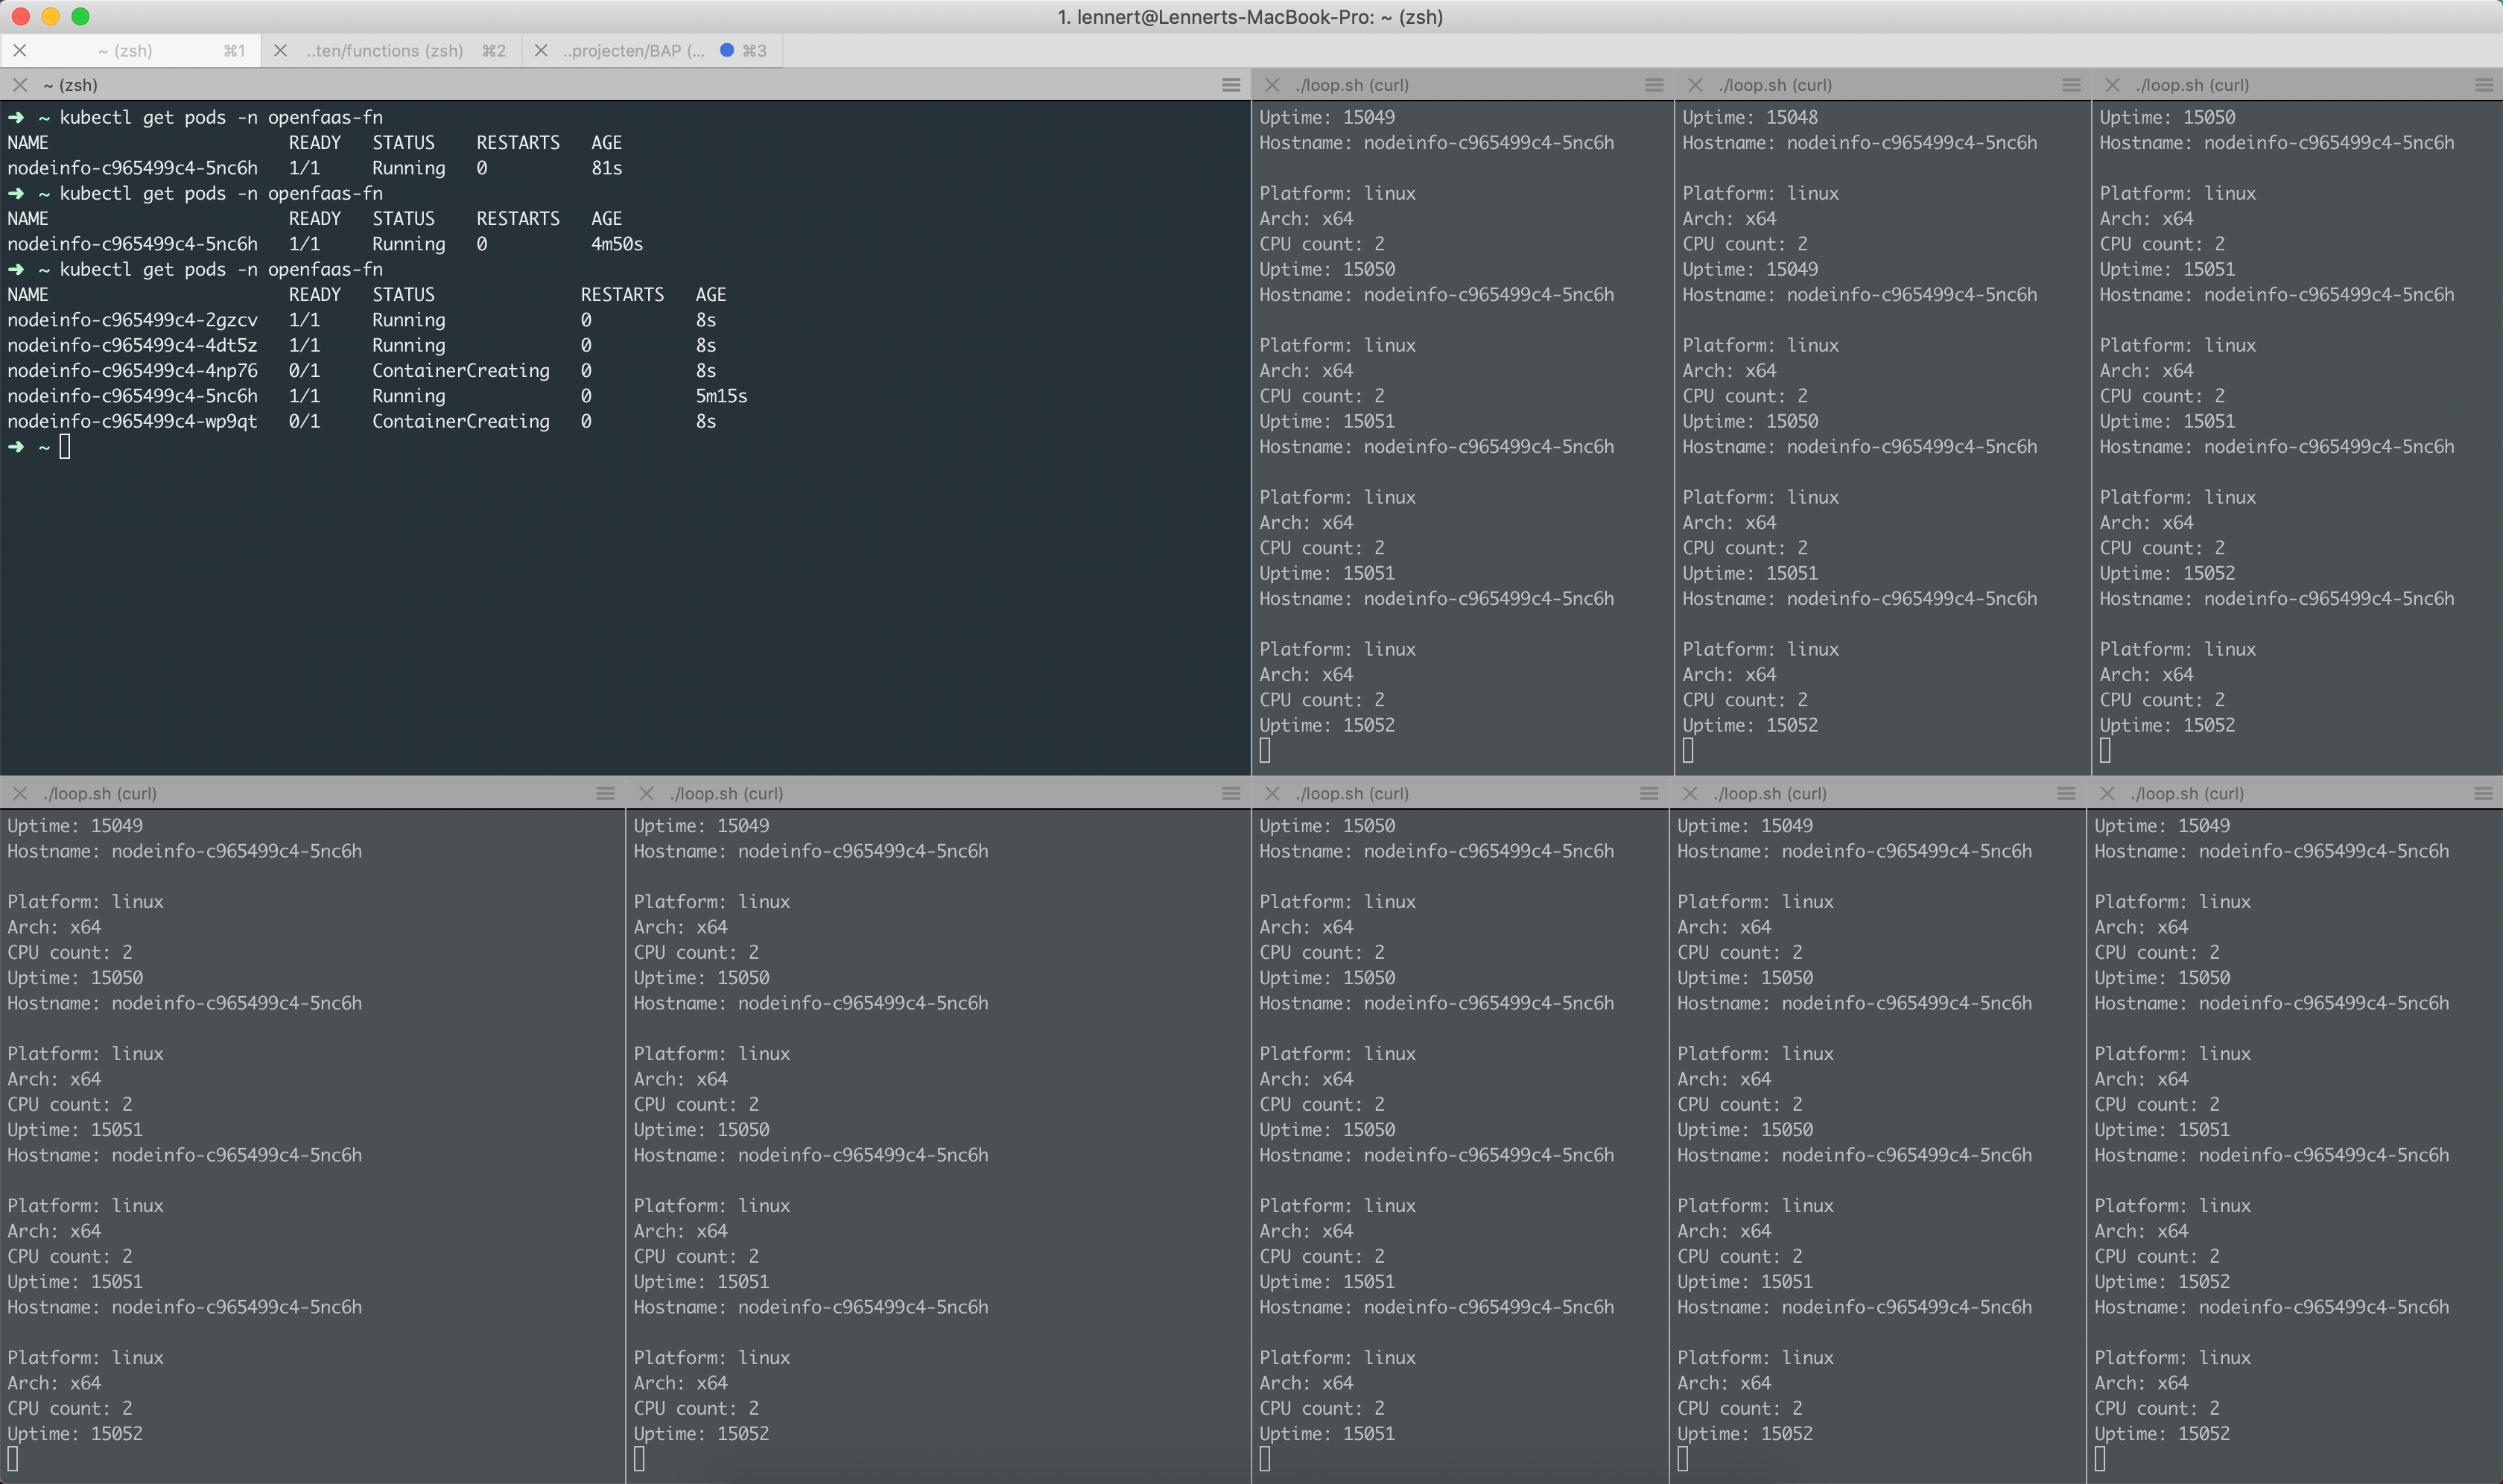
\includegraphics[width=1\textwidth]{img/openfaas-scalability-2.png}
    \caption{OpenFaaS opschalen pods na HTTP GET requests.}
    \label{fig:openfaas-scalability-2}  
\end{figure}

\begin{figure}
    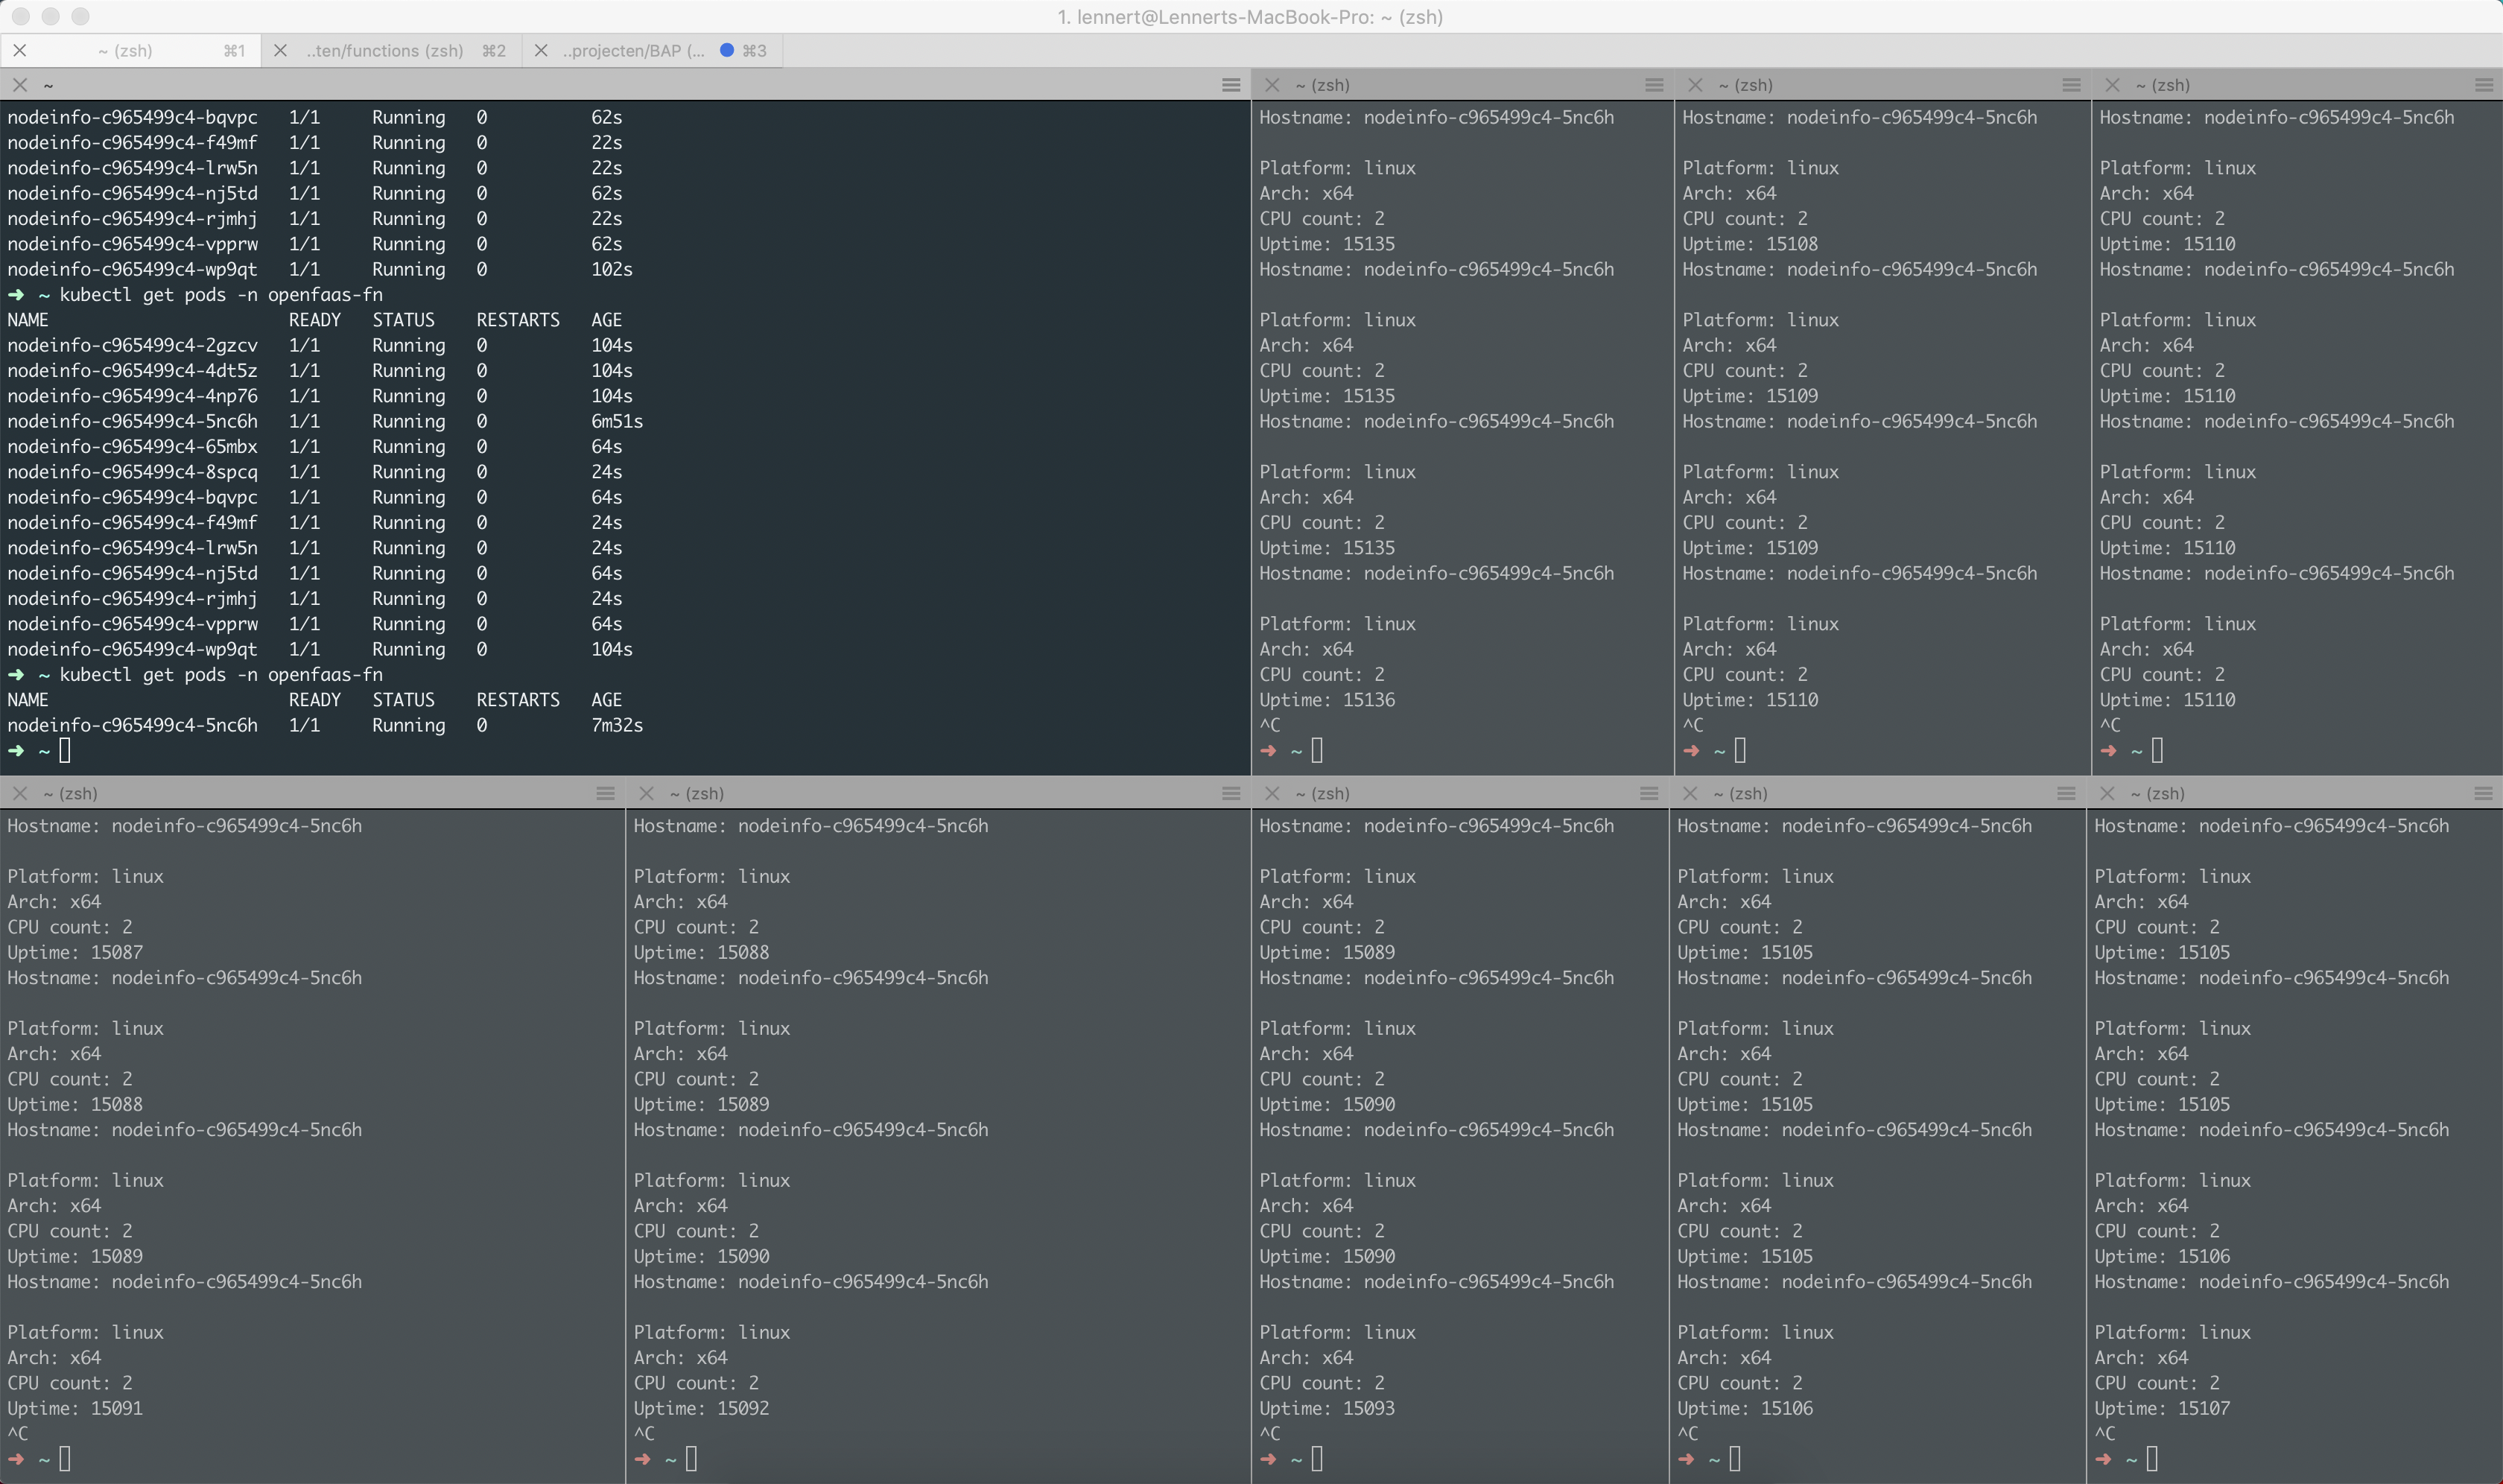
\includegraphics[width=1\textwidth]{img/openfaas-scalability-3.png}
    \caption{OpenFaaS pods schalen down wanneer requests worden afgebroken.}
    \label{fig:openfaas-scalability-3}  
\end{figure}

\subsection{Verzamelen functie gegevens}

\newpage
\section{Fission}
Het tweede framework dat onder de loep wordt genomen is Fission. Nubera gaf bij de start van dit onderzoek aan dat zij reeds geëxperimenteerd hadden met Fission en hier enige interesse voor hebben opgebouwd. Deze PoC bestaat dus enerzijds uit OpenFaaS, dat zelf gekozen werd als alternatief voor Fission, en Fission zelf. Aan het eind van dit onderzoek moet het duidelijk zijn waarin beide frameworks verschillen en welk het meest interessant zou kunnen zijn volgens de opgestelde requirements.

\subsection{Configuratie Minikube}
De configuratie voor Minikube is analoog aan diegene in sectie \ref{sec:configuratie-minikube}. Dezelfde stappen kunnen worden doorlopen om een werkende Minikube cluster op te zetten. Het is wel van belang dat de vorige Minikube installatie volledig wordt verwijderd eveneens als de Helm bestanden die werden aangemaakt tijdens de configuratie van vorige cluster, volgende commando's bereiken dit.

\begin{lstlisting}[language=bash]
$ minikube delete
$ cd ~
$ rm -rf .helm/ .minikube/
\end{lstlisting}

\subsection{Installatie Fission}
Fission kan worden geïnstalleerd als er een nieuwe Minikube cluster draait. De installatie werd geautomatiseerd in een shell script en is terug te vinden in bijlage \ref{sec:installatie-fission} onder de naam Installatiescript Fission. De installatie bestaat uit enkele stappen die rechtstreeks uit de documentatie\footnote{https://docs.fission.io/installation/} van Fission komen. Aan het installatiescript werden eveneens additionele stappen toegevoegd voor het opzetten van een Fission UI. Er werd gekozen voor de laatste stabiele versie van Fission, versie 1.2.0.

\subsection{Gebruik Fission}
\subsubsection{User Interface}
De installatie voorziet standaard geen meegeleverde user interface. Achteraf kan een UI worden geïnstalleerd maar deze blijkt echter niet te voldoen aan de verwachtingen. De GitHub repository\footnote{https://github.com/fission/fission-ui} waarvan de UI werd gedownload geeft eveneens aan dat deze zeker niet production ready is en momenteel nog een early alpha versie is. Het installatiescript exporteert een variabele met de link voor toegang tot de UI. De standaardpoort waarop de UI draait is poort 31319. In figuur \ref{fig:fission-ui} is te zien hoe de UI eruitziet. Wanneer de UI wordt geopend wordt er echter een foutboodschap weergegeven die luidt als volgt: ''Fission server supports API v2 only -- v1 is not supported. Please upgrade your Fission client/CLI''. Functies en environments die worden toegevoegd aan Fission worden niet weergegeven in de UI, het is ook niet mogelijk via de UI nieuwe componenten te definiëren. De UI werkt niet en dit is een known-issue op GitHub.
\begin{figure}
    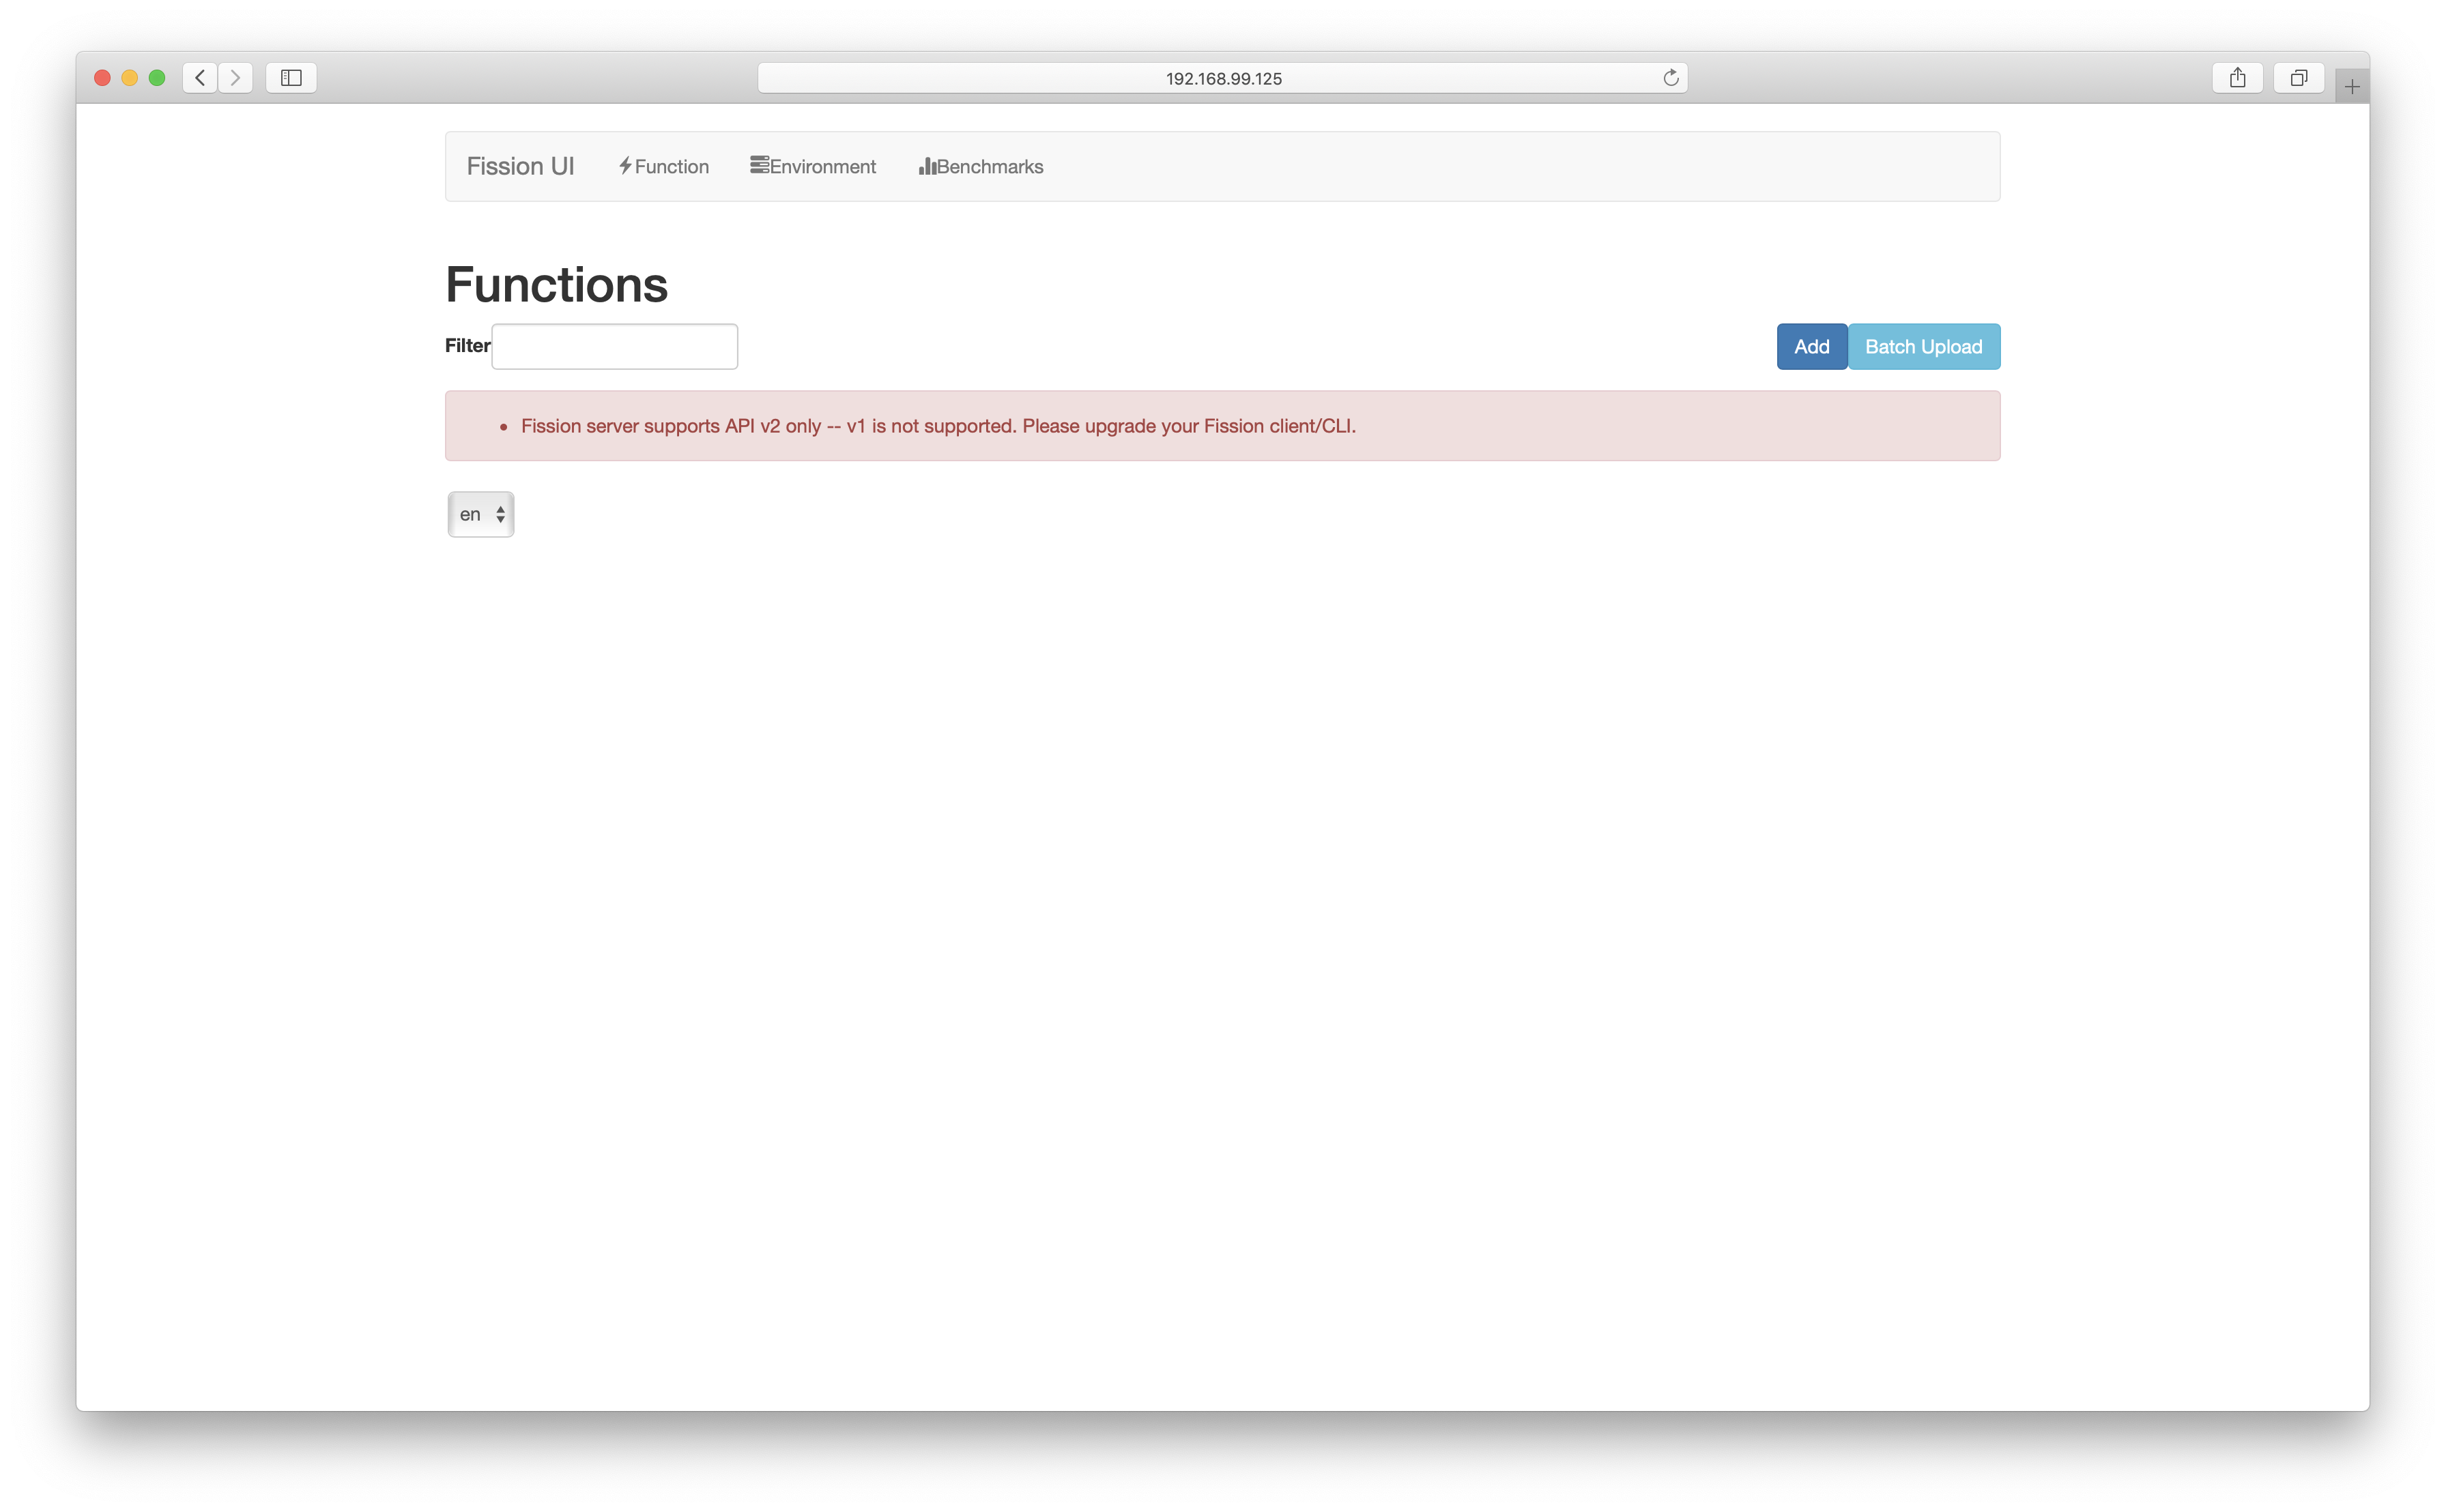
\includegraphics[width=1\textwidth]{img/fission-ui.png}
    \caption{Fission User Interface met foutmelding.}
    \label{fig:fission-ui}  
\end{figure}

\subsubsection{Command line tools}
Fission voorziet net zoals OpenFaaS command line tools voor het beheer van het framework. Via de CLI kunnen functies worden gedefinieerd, routes en environments gecreëerd, en triggers geconfigureerd. Alle taken en opdrachten worden uitgevoerd via de CLI. De CLI tools zijn eenvoudig in gebruik en in de documentatie worden goede voorbeelden voorzien om hiermee aan de slag te gaan. De werking van de CLI en de handelingen in Fission werden bestudeerd aan de hand van een boek over Serverless geschreven door \textcite{McKendrick2018}.

\subsubsection{Prometheus monitoring}
Prometheus wordt standaard voorzien in de installatie van Fission. Wanneer port forwarding wordt geactiveerd kunnen er queries worden verstuurd om metrics op te vragen via een webinterface. De code die de client voor querying activeert is hieronder beschreven, nadien kan de data worden opgevraagd via http://localhost:9090. Het is handig om via deze client verschillende queries uit te voeren om inzicht te krijgen in functies en hun performantie. Het is jammer dat er geen Grafana dashboard ''Out-of-the-box'' wordt meegeleverd om de prestaties van functies te visualiseren. Het is echter wel mogelijk om achteraf Grafana of een ander dashboard voor monitoring te installeren bovenop Istio (Dit wordt wel standaard met Fission meegeleverd). Omdat in voorgaande sectie omtrent OpenFaaS het Grafana dashboard al werd besproken, bespreken we hier de client voor Prometheus metrics querying.

\begin{lstlisting}[language=bash]
# Expose de Prometheus client via http://localhost:9090.
$ kubectl -n fission port-forward  \ 
$(kubectl -n fission get pod -l app=prometheus, \
component=server -o name) 9090
\end{lstlisting}

\subsection{Deployment demofunctie}
De werking hoe functies gedeployed worden is verschillend van OpenFaaS en vereist iets meer aandacht van de gebruiker. Initieel was de bedoeling om gebruik te maken van een Kubernetes secret om de credentials voor de Google API in op te slaan. Fission ondersteunde echter niet dezelfde acties als OpenFaaS en de secrets die werden gecreëerd konden niet op de gewenste manier in de functie worden gebruikt. Er werd geopteerd om daarom te werken met een private Docker image\footnote{https://cloud.docker.com/repository/docker/lennertmertens/python-env} die de nodige componenten zoals credentials en nodige pip packages bevat. De Docker image is gebaseerd op de standaard environment image die Fission aanbiedt.

\subsubsection{1. Aanmaak Docker image}
Het gebruik van een custom Python Docker image stelt gebruikers in staat deze te configureren naar eigen wensen en noden. De image kan worden gepubliceerd in een private repository voor veiligheidsoverwegingen. De onderdelen waaruit deze image is opgebouwd zijn hieronder opgesomd. De Docker image is gebaseerd op bestaande Docker files die werden ontwikkeld door de contributors van het Fission project, voor dit onderzoek werden de bestaande bestanden bewerkt, de link naar de code is steeds toegevoegd als voetnoot. De image kan eveneens worden gebouwd en worden opgeladen naar een Docker hub (of een andere) repository aan de hand van volgende commando's.

\begin{itemize}
    \item Dockerfile: in bijlage \ref{sec:dockerfile-fission} is de default Dockerfile\footnote{https://github.com/fission/fission/blob/master/environments/python/Dockerfile-2.7} te vinden die wordt voorzien in het Fission framework. Fission voorziet een aantal standaard images specifiek voor een aantal programmeertalen, deze images bevatten dependencies voor het uitvoeren van functies geschreven in een specifieke taal.
    \item Requirements.txt: Dit bestand bevat verschillende packets die met pip worden geïnstalleerd in de image. Standaard zijn er een aantal voorzien in de default Fission image. Er werden nog enkele extra packets toegevoegd voor het uitvoeren van de functie die zelf geschreven werd. Het bestand is terug te vinden in bijlage \ref{sec:requirements-fission}.
    \item Server.py\footnote{https://github.com/fission/fission/blob/master/environments/python/server.py}: Het Python script dat gekopieerd wordt naar de Docker image is een script dat werd geschreven door de medewerkers van het Fission project en zorgt ervoor dat functies die gebruik maken van deze image serverless kunnen worden aangeroepen. 
    \item Credentials.json: De Docker image bevat eveneens de credentials die werden aangemaakt voor gebruik van de Google API, deze zijn privé en voor elke gebruiker verschillend. Het credentials bestand dient in dezelfde map als de Dockerfile te worden geplaats zodat functies hiervan later gebruik kunnen van maken. 
\end{itemize}

\begin{lstlisting}[language=bash]
# Build de docker image vanuit de directory met de Dockerfile.
$ cd custom-docker-image
$ ls -l
total 40
-rw-r--r--  1 lennert  staff   257B May  6 18:03 Dockerfile
-rw-r--r--  1 lennert  staff   2.3K May  6 20:42 credentials.json
-rw-r--r--  1 lennert  staff   131B May  6 20:43 requirements.txt
-rw-r--r--  1 lennert  staff   4.0K May  6 17:34 server.py
# lennertmertens is de naam van de Docker Hub repository.
$ docker build -t lennertmertens/python-env . 
$ docker push lennertmertens/python-env
\end{lstlisting}

\subsubsection{2. Deploy functie}
Er is een verschil in werking in deployment van functies tussen Fission en OpenFaaS, Fission vereist een aantal additionele stappen die hieronder in detail worden doorlopen. Het is van belang dat alle pods die Fission aanmaakt beschikbaar zijn alvorens volgende stappen uit te voeren. Het duurt ongeveer een tweetal minuten, na installatie, tot alle pods beschikbaar zijn voor deployment van functies.
\\\\
Fission werkt by-default op een andere manier dan OpenFaaS. Wanneer een functie wordt gedeployed via OpenFaaS dan zal het framework steeds één container met de functie laten draaien, dit zorgt ervoor dat cold-starts niet kunnen voorkomen. Fission daarentegen zet containers die niet in gebruik zijn onmiddellijk af waardoor bij het aanroepen van functies cold-starts kunnen voorkomen en latency optreedt. Om beide frameworks op een gelijkwaardige manier te beoordelen wordt de instelling aangepast zodanig dat Fission ook steeds een container met de functie heeft draaien zodat cold-starts worden vermeden en de gegevens later met elkaar vergelijkbaar zijn. Om hetzelfde gedrag als bij OpenFaaS na te bootsen wordt er gebruik gemaakt van een Newdeploy executor zoals eerder besproken werd in sectie \ref{sec:fission-executors}. Volgende stappen maken het mogelijk om de Python demofunctie te deployen en beschikbaar te stellen via een URL langs de Fission router.

\begin{lstlisting}[language=bash]
# 1. Maak een environment aan waarin de Python functie zal 
# worden uitgevoerd, de environment wordt opgesteld met 
# de eerder gemaakte Docker image.
$ fission environment create --name python-env \
--image lennertmertens/python-env

# 2. Deploy de geschreven Python functie (cd in de 
# directory met de Python code).
# Stel eveneens in dat er minimum een pod draait met de functie.
$ fission function create --name serverless-demo \
--code handler.py --env python-env \
--minscale 1 --executortype newdeploy

# 3. Voeg een pad toe voor toegang via de Fission router.
$ fission route create --function serverless-demo --url /serverless-demo
\end{lstlisting}
 
\subsubsection{handler.py}
Handler.py is het Python script dat geschreven werd in sectie \ref{sec:demofunctie} en werd aangepast specifiek voor Fission. De manier waarop functies in Fission worden aangeroepen is verschillend van OpenFaaS. De functies hebben een main methode nodig om uitvoerbaar te zijn, daarom dat de aanpassingen werden aangebracht. De Fission functie maakt eveneens gebruik van credentials die aanwezig zijn in de Docker container. Het Python script dat wordt gedeployed op het Fission framework is terug te vinden in bijlage \ref{sec:demofunctie-fission}.

\subsection{Uitvoeren demofunctie}
De demofunctie reageert op HTTP GET requests, deze actie kan worden getriggered op verschillende manieren. Fission voorziet in de command line tools een commando voor het testen van functies die gedeployed werden op het framework. De output van het test commando weergeeft logs en kan gebruikt worden voor het troubleshooten van functies. Tijdens het deployen van de demofunctie werd er eveneens een pad voor de functie gedefinieerd, via de Fission router en het aangemaakte pad kan de functie ook worden aangeroepen. Gebruikers kunnen naar het IP adres van de router surfen gevolgd door het pad of kunnen aan de hand van een curl commando de functie opvragen.

\begin{lstlisting}[language=bash]
# Aanroep functie met test commando.
$ fission function test --name demo-functie
# Aanroep functie met curl.
$ curl http://$FISSION_ROUTER/serverless-demo
\end{lstlisting}

\subsection{Schaalbaarheid Fission}
Om de schaalbaarheid van Fission te demonstreren wordt er gebruik gemaakt van een demofunctie die terug te vinden is in de Fission repository op GitHub, onder de naam hello.js\footnote{https://github.com/fission/fission/blob/master/examples/nodejs/hello.js}. De demofunctie die hier wordt gebruikt is een simpele Hello World applicatie geschreven in Node.js. Alvorens er getest kan worden op schaalbaarheid wordt de functie op analoge manier gedeployed als de demofunctie die in Python geschreven werd. Er moet eerst wel een Node.js environment worden aangemaakt en bij het definiëren wordt gekozen voor een minscale van 1 en een Newdeploy executor om automatische schaalbaarheid te voorzien. De stappen om de omgeving klaar te zetten zijn hieronder beschreven. Wanneer de load te zwaar wordt voor één pod om deze te verwerken dan zullen er additionele functie pods worden aangemaakt en wordt er automatisch load balancing tussen de functie pods voorzien.

\begin{lstlisting}[language=bash]
# 1. Aanmaak Node.js environment.
$ fission environment create --name node-env \
--image fission/node-env

# 2. Deploy de hello.js functie.
$ fission function create --name hello \
--code hello.js --env node-env \
--minscale 1 --executortype newdeploy

# 3. Maak een route voor de functie.
$ fission route create --function hello --url /hello
\end{lstlisting}

----TO BE ADDED -----

\subsection{Verzamelen functie gegevens}
Om een grondige vergelijking tussen beide frameworks te maken is het interessant inzicht te hebben in de performance verschillen tussen beiden. De Python demofunctie die werd geschreven schrijft de tijd weg die nodig is voor het uitvoeren van de functie naar een bestand in Google spreadsheets. De eerste meting weergeeft enkel de tijd die de functie nodig heeft om de code uit te voeren. De functie die op Fission werd gedeployed, wordt net zoals bij OpenFaaS tweehonderd keer aangeroepen door middel van een loop. De resultaten die worden weggeschreven naar de spreadsheet zullen later met elkaar worden vergeleken. In bijlage \ref{sec:demofunctie-uitvoeringstijd} zijn de resultaten van de uitvoeringstijd van de functie (de code zelf) terug te vinden. 
\\\\
In de veronderstelling dat de uitvoeringstijd, van enkel en alleen de code, tussen de twee frameworks niet veel zou verschillen werd er nog een tweede test gemaakt. De tweede test meet de volledige tijd vanaf dat er een HTTP request wordt verzonden met het ''curl'' commando, tot er een response met de overeenkomstige tijd wordt ontvangen. De uitvoeringstijd of de looptijd van de volledige functie wordt weggeschreven naar een lokaal bestand. Voor elk framework wordt er een apart bestand aangemaakt. In het hoofdstuk \ref{ch:vergelijking-frameworks} zullen op basis van de requirements en de uitgevoerde metingen beide frameworks met elkaar worden vergeleken. Het bestand met de volledige looptijd van de functies is terug te vinden in bijlage \ref{sec:demofunctie-volledige-looptijd}.

\begin{lstlisting}[language=bash]
#!/bin/bash
touch looptijd-functie-fission.csv
for i in {1..200};
do
  curl -s -w "%{time_total}\n" -o \
  /dev/null http://$FISSION_ROUTER/serverless  \
  >> looptijd-functie-fission.csv
done
\end{lstlisting}
